\documentclass[../deliverable-two.tex]{subfiles}

\begin{document}
\label{diagrams}

\subsection{Diagramy stanów}

\subsubsection{Maszyna wirtualna}
Najważniejszym obiektem biznesowym w systemie jest maszyna wirtualna, do której będą podłączać się użytkownicy.

\begin{figure}[!h]
	
	\centering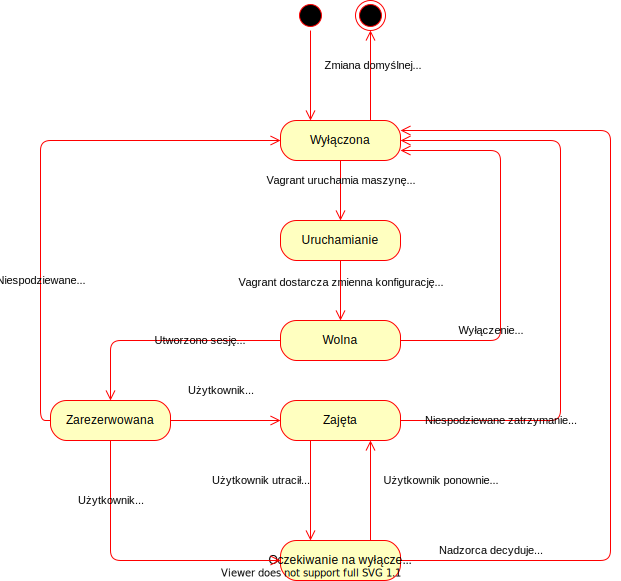
\includegraphics[width=\screenswidth]{state_diagrams/virtual_machine.png}
	
	\vskip-1.5ex
	
	\caption{Diagram stanów dla maszyny wirtualnej}
	\label{state_vm}
\end{figure}

Maszyna aby być całkowicie uruchomiona musi być zaopatrzona we wszystkie konfiguracje.
Stan "Wolna" oznacza możliwość przypisania sesji do tej maszyny w razie potrzeby.
Po rezerwacji użytkownik nie musi od razu się zalogować (posiada pewien czas na podłączenie się do systemu).
Maszyna przy oczekiwaniu na podłączenie sie uzytkownika (różwnież po zerwaniu połączenia) oczekuje w stanie "Oczekiwanie na wyłączenie maszyny".
Gdy użytkownik pracuje na maszynie (wiemy o tym przez monitorowanie kolejki zdefiniowanej ) 

\subsection{Diagramy aktywności}

\subsection{Diagramy klas}

\subsection{Diagramy sekwencji}

\end{document}